\section{磁気スーパーミラー}
磁気スーパーミラーは入射した中性子のうちスピン上向きのみを選択的に取り出す役割を持つ。膜厚を少しずつ変えた多層膜により全反射とBragg反射の両方を利用して幅広いエネルギーの中性子を反射することができる。反射の詳しい原理は\ref{mirror_sec}章で述べる。

\begin{figure}[H]
\centering
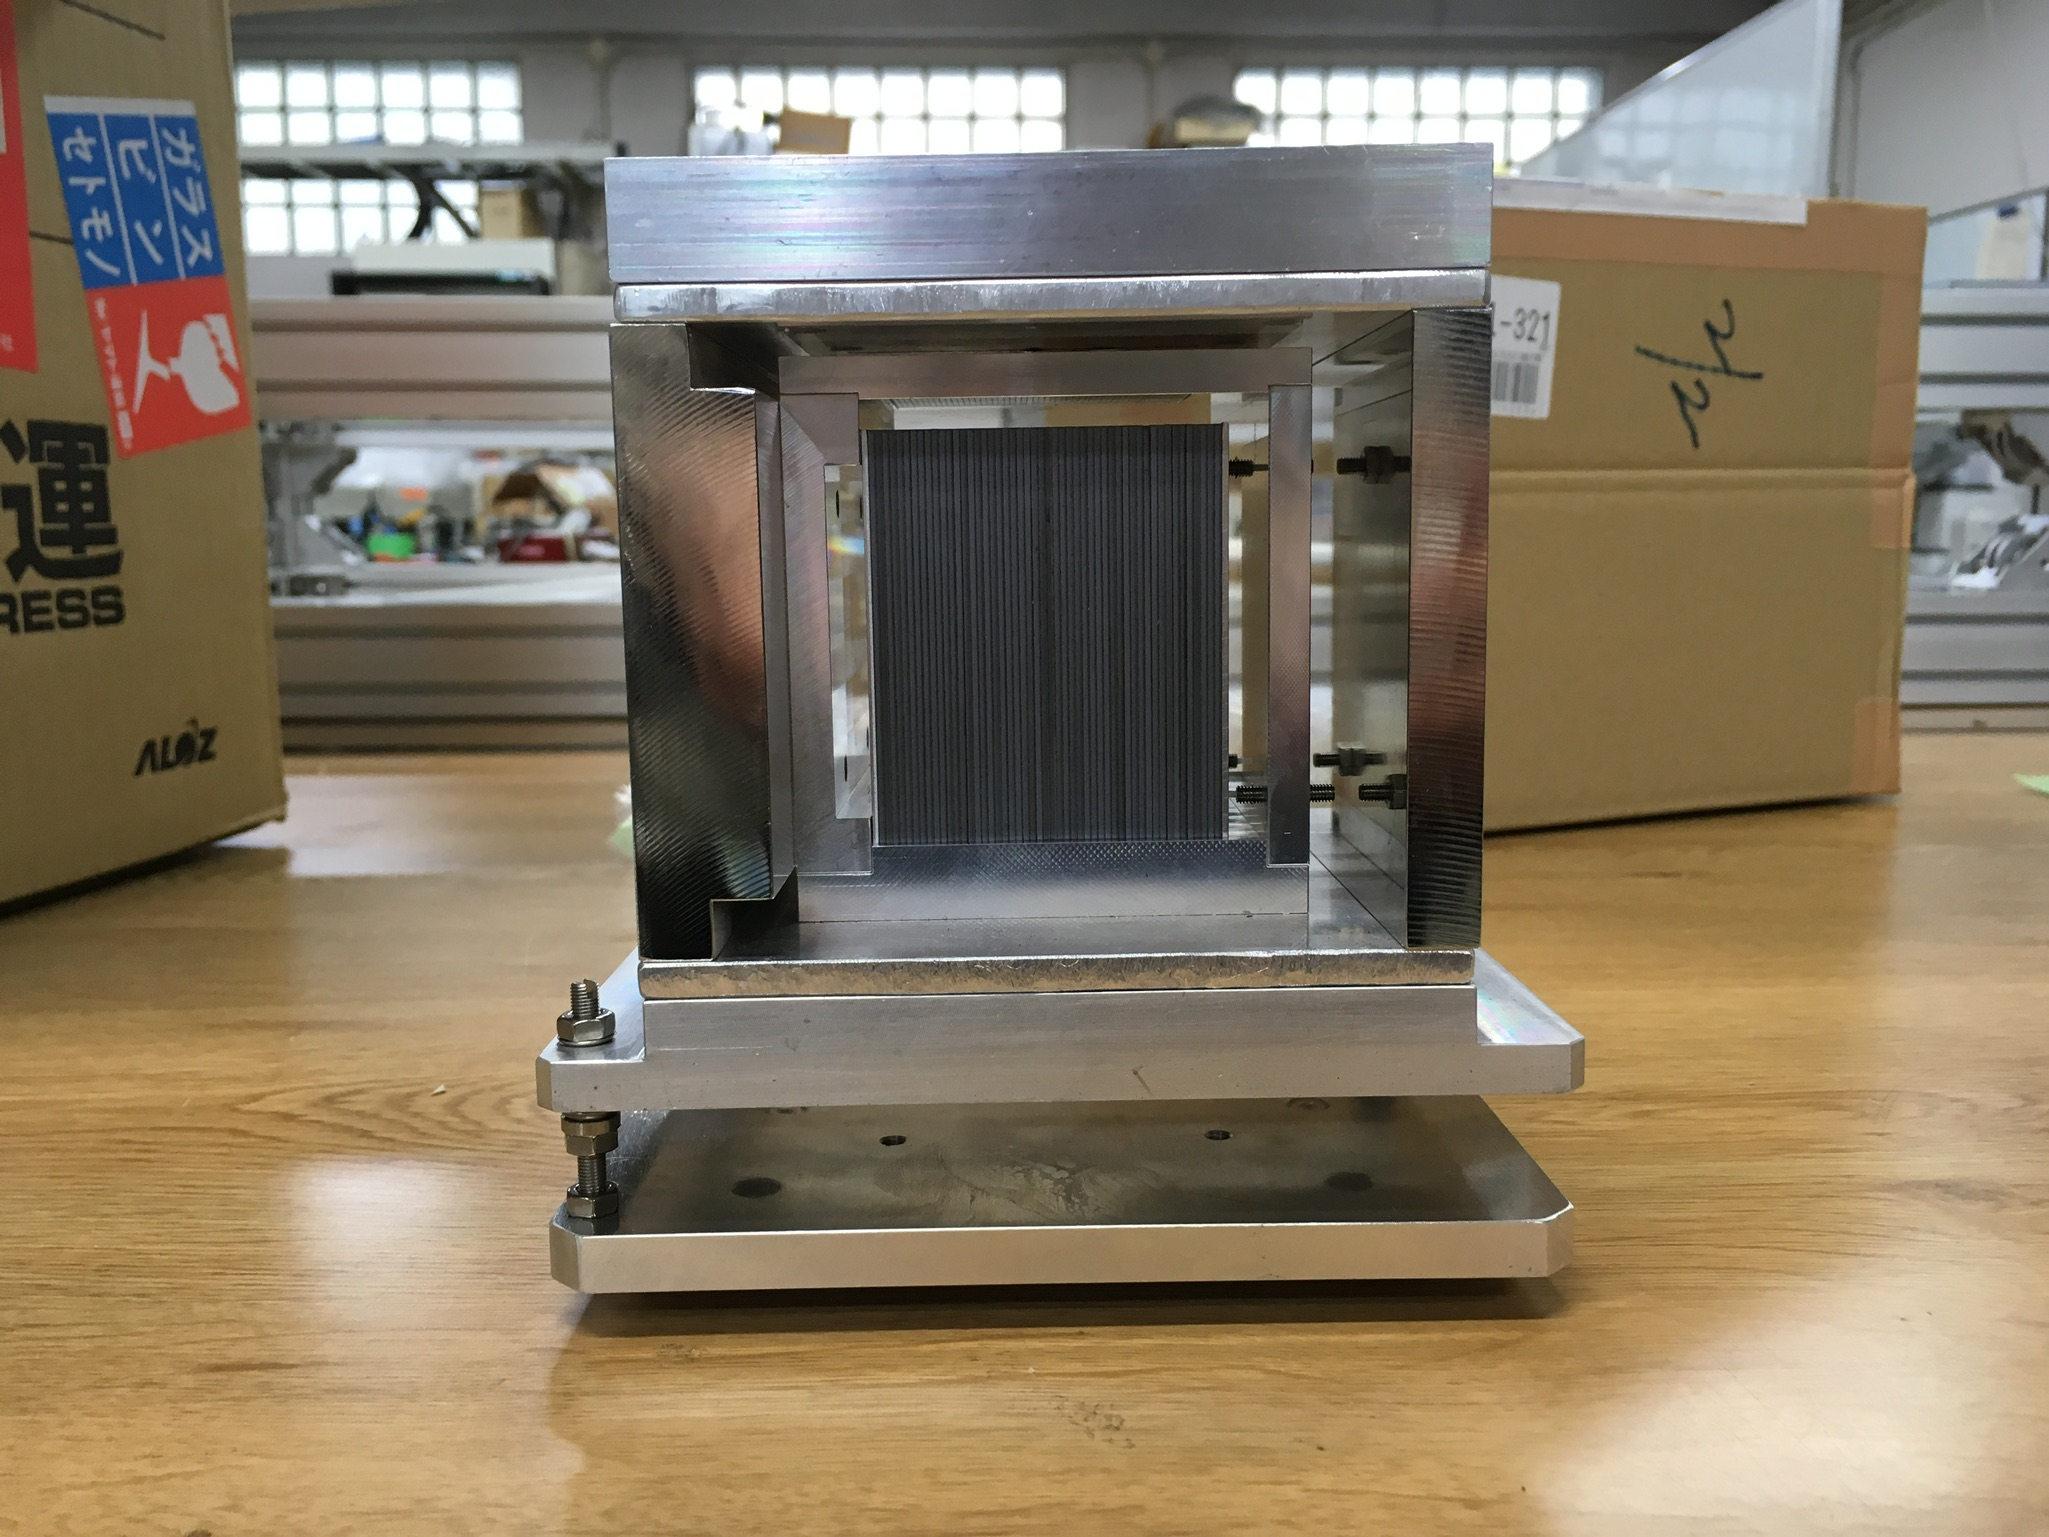
\includegraphics[width=8cm]{device/mirrorphoto.jpg}\caption{磁気スーパーミラー}
\end{figure}